\documentclass[a4paper]{article}
\usepackage[utf8]{inputenc}
\usepackage{fullpage}
\usepackage{graphicx}
\usepackage{amsmath}
\usepackage{wrapfig}
\usepackage{float}
\usepackage{hyperref}
\usepackage{verbatim}
\usepackage{lmodern}
\usepackage[most]{tcolorbox}
\usepackage{authblk}
\usepackage{csquotes}


\renewcommand{\familydefault}{\sfdefault}

% Set up the way you show hyperlinks
\hypersetup{colorlinks=true, linkcolor=blue, filecolor=magenta, urlcolor=cyan}

% Verbatim environment
\tcbset{
    frame code ={},
    center title,
    left=0pt,
    right=0pt,
    top=0pt,
    bottom=0pt,
    colback=gray!19,
    colframe=white,
    width=\dimexpr\textwidth\relax,
    enlarge left by =0mm,
    boxsep=5pt,
    arc=0pt,
    outer arc=0pt
    }

\title{\textbf{How to create a Forcefield}}
\date{}

% REFERENCE ME PLS
\author[1]{Jérôme Rihon}
\affil[1]{\small KU Leuven, Rega Institute for Medical Research, Medicinal Chemistry , Herestraat 49 - Box 1041, 3000 Leuven, Belgium}


\begin{document}

\maketitle

\tableofcontents

\pagebreak

\footnotesize
\section{Start a prep file}


\subsection{Standard file format}
Documentation is found here : \href{https://ambermd.org/doc/prep.html}{ambermd.org/doc/prep.html}\\
Prep files consists of the following make :\\
\textit{The parts in between single quotes are condensed bits of information of the keywords on that line.}
\scriptsize
\begin{tcolorbox}
\begin{verbatim}
 0 0 2                                  'Generally, only a value 2 is required, for ALL ATOM MODELS'
                                        'Leave this line purposefully blank!'
MORPHOLINO-ADENINE                      'This is a remark line; name of the molecule for the database purposes'
MA.res                                  'Residue name in the pdb. Standard here is "molecule.res" '
MA INT 1                                'Residue, Internal Coordinates, binary format output '
CORRECT OMIT DU BEG                     'Correct order of internal coordinates; delete beginning dummy atoms'
0.000                                   'Set to 0.00 and make explicit loop closing bond statements'
   1  DUMM  DU    M    0  -1  -2     0.000    0.00        0.00    .00000
   2  DUMM  DU    M    1   0  -1     1.000    0.00        0.00    .00000
   3  DUMM  DU    M    2   1   0     1.000   90.00        0.00    .00000


IMPROPER                                'Denote which atoms are important when considering improper dihedrals,
                                            always a set of four atoms. Improper torsions are used to keep
                                            the asymmetric centers from racemizing in the united atom model
                                            where all the C-H hydrogens are omitted.
                                            They can also be used to enforce planarity.'


LOOP CLOSING EXPLICIT                   'Depending on the main atoms, which ones are loop closing.
                                            So which ones close the ring system according to the atoms denoted.
                                            Here you only required to add a set of two atoms at a time.'

CHARGE                                  'Override any charges from the dataframe'

DONE                                    'Last line of the molecule's information'
STOP                                    'Only add a stop statement if this is the final molecule in your file
                                            this is needed as the prep file is read in as an infinite loop.'
\end{verbatim}
\end{tcolorbox}
\footnotesize

\vspace{3mm}
\noindent Sidenote for improper dihedrals. These are of special interest when designing and defining the nucleobase moiety, as all substituents on it are very likely to be flattened for the simulation.
\scriptsize
\begin{tcolorbox}
\begin{verbatim}
An IMPROPER torsion is any torsion where a set of four atoms are not bonded consecutively.
Improper torsions are used to keep the asymmetric centers from racemizing in the united atom model
    where all the C-H hydrogens are omitted.
They can also be used to enforce planarity. Especially interesting for nucleobases.

The standard case is:

    where the central atom (K) is the third (3rd) atom in the improper                      J
    and the order of the other three is determined alphabetically                           |
    by atom type and if types are the same by atom number.                                  K
    The improper torsions should be defined in such a way that                             / \
    the proper torsions are not duplicated. The atoms making the following -->            I   L

                                                                                    Improper I-J-K-L
\end{verbatim}
\end{tcolorbox}
\subsection{Tree Structure - Topological Types}\label{sec:ambertree}
\footnotesize
\begin{itemize}
    \item \textbf{DU} Dummy atoms; PREP requires that three dummy atoms precede the actual atoms of the residue. These atoms are simply used to define the orthogonal space axis for the residue.
    \item \textbf{M} Main; Main atoms describe the principal "path" through the residue, starting at the connection to the previous residue and ending at the connection to the next  residue.
    \item \textbf{B} Branch; An atom that must have a total of three (3) connections
    \item \textbf{S} Side; An atom that must have a total of two (2) connections to  other  atoms
    \item \textbf{E} End ; An atom that has only one (1) connection to other atoms,  thus is the `dead end` of the tree structure.
    \item \textbf{3, 4, 5, 6} A "3"-type atom has four connections, and the rest follows the series (ascending amount of possible bonds). For most organic molecules, unless interesting protonation states occur (that are not defined by other names) or intense dative bonding, except for "3", this is not really employed too much.
\end{itemize}

\subsection{AMBER Atom Typing}
Extensive documentation on atom typing can be found in Section \ref{sec:atomtyping} of this manual.
\subsection{Prep File Structure}

\footnotesize
\begin{center}
\begin{tabular}{ c c c c c c c c c c c }
\hline
 Index & Name of Atom & AmbFFname & Top. Type &   CONECT1 &   CONECT2 &   CONECT3 &    Bond  &     Angle & Dihedral  &    Charge \\
\hline
 1 &       DUMM   &        DU &        M  &        0  &       -1  &       -2  &    0.00  &     0.00  &     0.00  &    0.0000 \\
 2 &       DUMM   &        DU &        M  &        1  &        0  &       -1  &    1.00  &     0.00  &     0.00  &    0.0000 \\
 3 &       DUMM   &        DU &        M  &        2  &        1  &        0  &    1.00  &    90.00  &     0.00  &    0.0000 \\
 4 &        H6T   &        HO &        M  &        3  &        2  &        1  &    1.00  &    90.00  &   180.00  &    0.4532 \\
 5 &        O6'   &        HO &        M  &        4  &        3  &        2  &    1.00  &   110.00  &   180.00  &   -0.6862 \\
 6 &        C6'   &        CI &        M  &        5  &        4  &        3  &    1.40  &   110.00  &   180.00  &    0.0279 \\
 7 &        H6'   &        H1 &        E  &        6  &        4  &        3  &    1.00  &   110.00  &   -60.00  &    0.0773 \\
 \ldots & \ldots & \ldots & \ldots & \ldots & \ldots & \ldots & \ldots & \ldots & \ldots & \ldots\\
11 &        O5'   &        OS &        S  &        9  &        6  &        5  &    1.40  &   110.00  &    60.00  &   -0.3487 \\
 \ldots & \ldots & \ldots & \ldots & \ldots & \ldots & \ldots & \ldots & \ldots & \ldots & \ldots\\
\hline
\end{tabular}
\end{center}
\footnotesize

\begin{itemize}
    \item Add only a single line between the required table and the extra optional statements (CHARGE, LOOP, IMPROPER, DONE).
    \item \textbf{NB} The Bond, Angle and Dihedral column is typically what is known as a Z-matrix or a set of Internal Coordinates \href{https://en.wikipedia.org/wiki/Z-matrix_(chemistry)}{Z-matrix wikipedia page}.
    \item When the (INT) keyword is used, PREP reads but disregards the connectivities and bond, angle and dihedral columns when supplied with a model structure. We use this to our advantage, since we already have a given model instead trying to generate it through tLEaP (which is what the z-matrix is for).
\end{itemize}

\subsection{Atom type tree and structure}
The following figure shows an depiction of the textfile contents of \verb PATH/TO/AMBER/amber18/dat/leap/prep/nucleic10.in \\
\begin{figure}[h!]
    \centering
    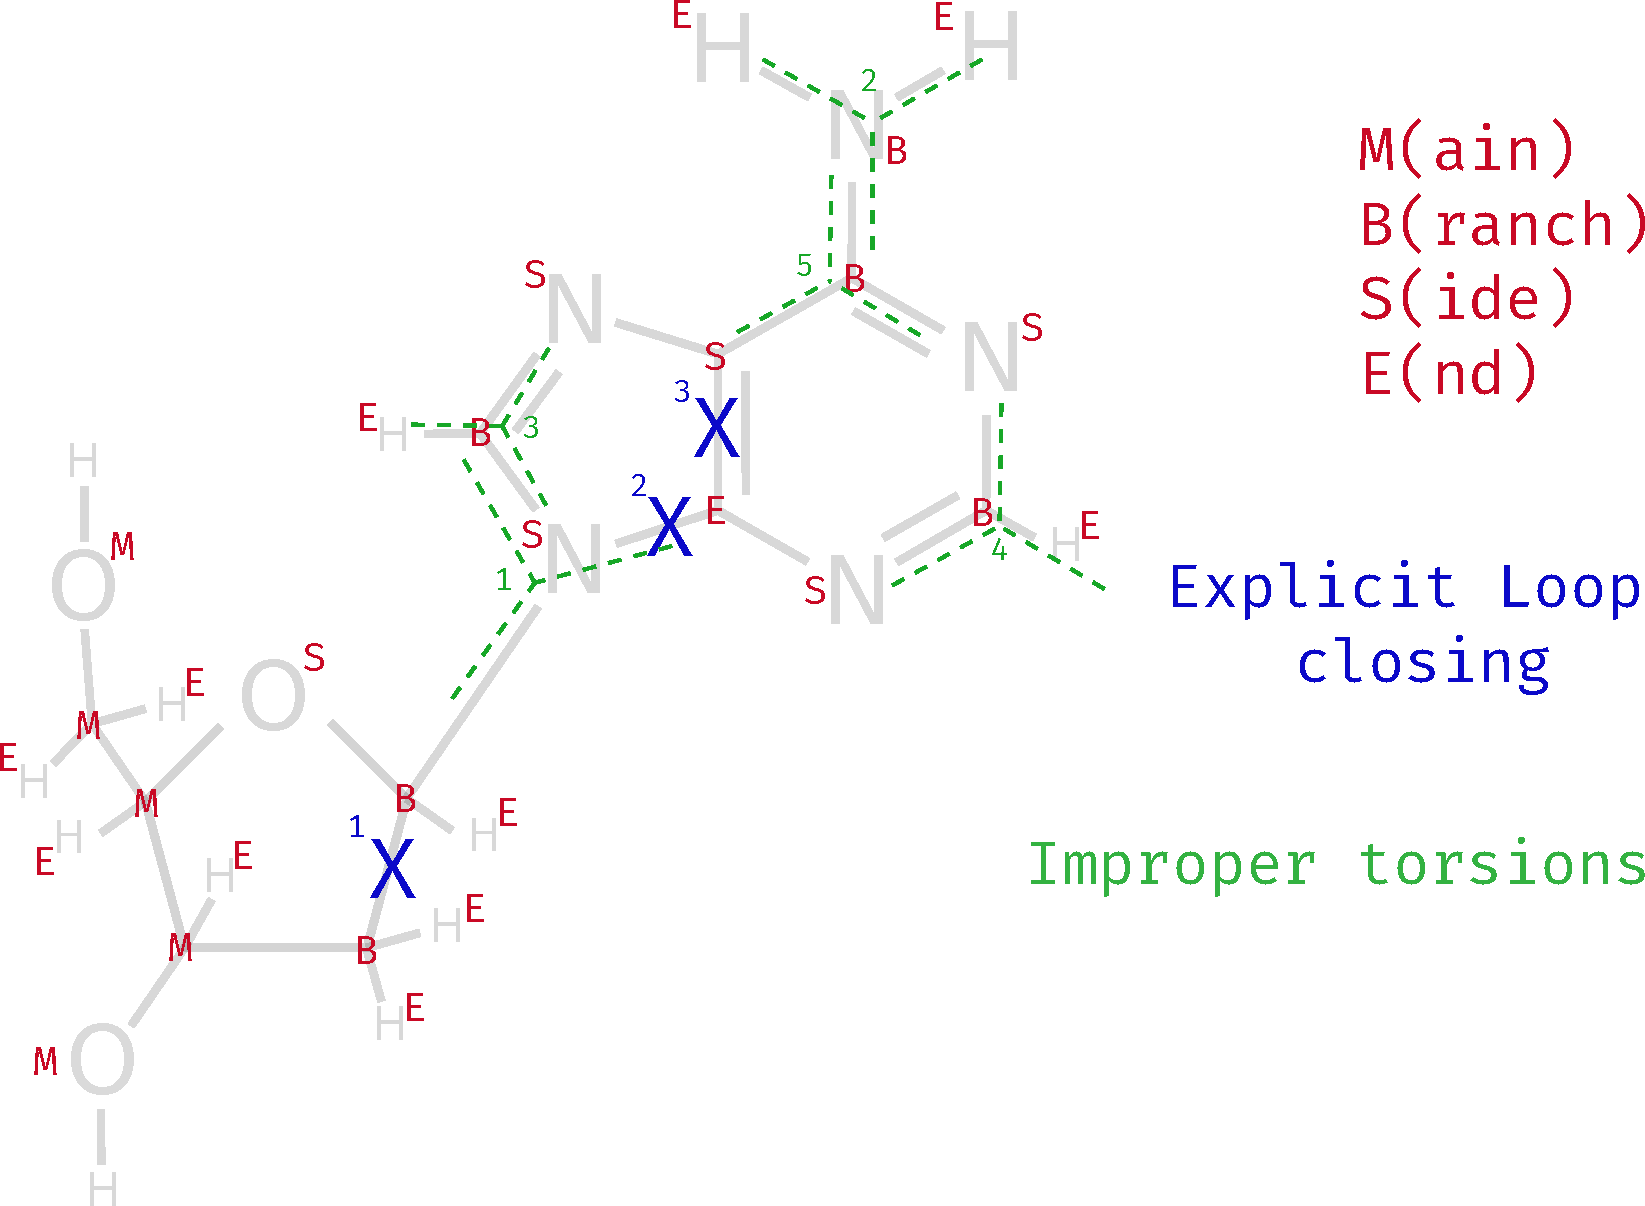
\includegraphics[width=0.79\textwidth, keepaspectratio]{./figures/prepfile_atomtype_tree.pdf}
\end{figure}
%
%
%
\pagebreak
%
%

\noindent Here is an example of what a prep file can look like : 
\begin{tcolorbox}
\begin{verbatim}
    1    0    2

db94.dat
D-ADENOSINE - with 5' - OH end group and 3' - O(minus)

 DA5  INT     1
 CORRECT NOMIT DU   BEG
   0.0
   1   DUMM  DU    M    0  -1  -2    0.00      0.00      0.00       0.0000
   2   DUMM  DU    M    1   0  -1    1.00      0.00      0.00       0.0000
   3   DUMM  DU    M    2   1   0    1.00     90.00      0.00       0.0000
   4   HO5'  HO    M    3   2   1    1.00    120.00    180.00       0.4422
   5   O5'   OH    M    4   3   2    0.96    101.43    -98.89      -0.6318
   6   C5'   CI    M    5   4   3    1.44    119.00    -39.22      -0.0069
   7   H5'   H1    E    6   5   4    1.09    109.50     60.00       0.0754
   8   H5''  H1    E    6   5   4    1.09    109.50    -60.00       0.0754
   9   C4'   CT    M    6   5   4    1.52    110.00    180.00       0.1629
  10   H4'   H1    E    9   6   5    1.09    109.50   -200.00       0.1176
  11   O4'   OS    S    9   6   5    1.46    108.86    -86.31      -0.3691
  12   C1'   CT    B   11   9   6    1.42    110.04    105.60       0.0431
  13   H1'   H2    E   12  11   9    1.09    109.50   -240.00       0.1838
  14   N9    N*    S   12  11   9    1.52    109.59   -127.70      -0.0268
  15   C8    CK    B   14  12  11    1.37    131.20     81.59       0.1607
  16   H8    H5    E   15  14  12    1.08    120.00      0.00       0.1877
  17   N7    NB    S   15  14  12    1.30    113.93    177.00      -0.6175
  18   C5    CB    S   17  15  14    1.39    104.00      0.00       0.0725
  19   C6    CA    B   18  17  15    1.40    132.42    180.00       0.6897
  20   N6    N2    B   19  18  17    1.34    123.50      0.00      -0.9123
  21   H61   H     E   20  19  18    1.01    120.00    180.00       0.4167
  22   H62   H     E   20  19  18    1.01    120.00      0.00       0.4167
  23   N1    NC    S   19  18  17    1.34    117.43    180.00      -0.7624
  24   C2    CQ    B   23  19  18    1.33    118.80      0.00       0.5716
  25   H2    H5    E   24  23  19    1.08    120.00    180.00       0.0598
  26   N3    NC    S   24  23  19    1.32    129.17      0.00      -0.7417
  27   C4    CB    E   26  24  23    1.35    110.80      0.00       0.3800
  28   C3'   CT    M    9   6   5    1.53    115.78   -329.11       0.0713
  29   H3'   H1    E   28   9   6    1.09    109.50     30.00       0.0985
  30   C2'   CT    B   28   9   6    1.53    102.80    -86.30      -0.0854
  31   H2'   HC    E   30  28   9    1.09    109.50    120.00       0.0718
  32   H2''  HC    E   30  28   9    1.09    109.50    240.00       0.0718
  33   O3'   OS    M   28   9   6    1.42    116.52   -203.47      -0.5232

IMPROPER
 C8   C4   N9   C1'
 C6   H61  N6   H62 
 N7   N9   C8   H8
 N1   N3   C2   H2
 C5   N1   C6   N6

LOOP CLOSING EXPLICIT
 C1'  C2'
 C4   C5
 C4   N9

DONE
\end{verbatim}
\end{tcolorbox}
\pagebreak


%
%
%
%
%
%
%
%
%
%
%
%
%
%
%
%
%
%
%
%
%
%
%
%
%
%
%
%
%
%
\section{RESP Charge derivation}
\subsection{The R.E.D server}
The R.E.D. server is a tool to automate the RESP charge derivation. However you'd want to derive RESP charges is up to you. One can easily do it on their local system and doing it manually gives you a very good understanding of it all (see \ref{sec:resplocal}).\\
The R.E.D. server will run geometry optimisations of your molecule before calculating the atomic charges. This optimisation is by far the most expensive step of it all.
It is advisable to add an extensive \verb system.config  and a \verb project.config  to your inputs, to optimise the accuracy of your calculations.\\
\\
The R.E.D. server does not need registration.\\
Computational chemistry available through the following packages : 
\begin{itemize}
\item Gaussian (Advisable to stick to this software! Commonly used in the AMBER community)
\item GAMESS-US
\item Firefly
\item RESP
\item \href{https://upjv.q4md-forcefieldtools.org/REDServer-Development/news.php}{R.E.D Server Development news}
\end{itemize}
%
\subsubsection{R.E.D server documentation}\label{sec:reddocs}
Read these publications as they contain a quite some information.
\begin{itemize}
    \item Documentation of the RESP charge derivation : \textit{A Well-Behaved Electrostatic Potential Based Method Using Charge Restraints for Deriving Atomic Charges: The RESP Model} \href{https://pubs.acs.org/doi/10.1021/j100142a004}{RESP publication; Bayly et al.}
    \item Documentation of the R.E.D server : \textit{R.E.D. Server: a web service for deriving RESP and ESP charges and building force field libraries for new molecules and molecular fragments} \href{https://pubmed.ncbi.nlm.nih.gov/21609950/}{R.E.D Server publication; Vanquelef et al}
    \item Improvements on the R.E.D server : \textit{The R.E.D. tools: advances in RESP and ESP charge derivation and force field library building} \href{https://pubs.rsc.org/en/content/articlelanding/2010/cp/c0cp00111b}{R.E.D tools publicationDupradeau et al.}
    \item PyRed stable interface \href{https://upjv.q4md-forcefieldtools.org/REDServer-Development/}{PyRed server}
    \item R.E.D Server homepage : \href{https://upjv.q4md-forcefieldtools.org/}{Homepage QM4Forcefieldtools}
    \item Here you can find how to prepare input files for a first R.E.D Server development : \href{https://upjv.q4md-forcefieldtools.org/Tutorial/Mini-HowTo-InputFiles.pdf}{Inputfile preparation HowTo} \end{itemize}

\subsubsection{Basics}
The tutorials of the R.E.D server contain a section on how the RESP derivation scheme works. This can help one with understanding how restraints and equivalencing works, either through the server or on the local system.\\
Be sure to check out the \textbf{Tutorial : \href{https://upjv.q4md-forcefieldtools.org/Tutorial/Tutorial-4.php}{Updated Tutorial} !}


\subsubsection{Configuration files}
The following files are required to run a R.E.D. server job :
\begin{itemize}
    \item System.config \href{https://upjv.q4md-forcefieldtools.org/REDServer-Development/Documentation/System.config}{Link to System.config}
    \item Project.config \href{https://upjv.q4md-forcefieldtools.org/REDServer-Development/Documentation/Project.config}{Link to Project.config}
    \item Some added information on the format of the input files \href{https://upjv.q4md-forcefieldtools.org/REDServer-Development/Documentation/readme.txt}{README HowTo}
\end{itemize}
\vspace{3mm}
\noindent Everything here should guide you to be able to manage and generate a very simple charge derivation that is compatible with AMBER, GROMACS, OPLS or CHARMM.\\
\pagebreak
%
%
%
%
%
%
%
%
%
%
%
%
%
%
%
%
%
%
%
%
%
%
%
%
%
%
%
%
%
%
\subsection{RESP charge derivation on your local system}\label{sec:resplocal}

\subsubsection{Small set-up and reasoning behind the RESP calculation}\label{sec:respdocs}
The ORCA manual, available on their repository over at \href{https://orcaforum.kofo.mpg.de/app.php/portal}{ORCA Forum}. You will have to make a free account and then you get access to the Downloads page and there are several folders. Download the latest version of ORCA, together with the respective version of Open MPI, also free of charge \href{https://www.open-mpi.org/}{Open MPI official homepage}. Installing ORCA is easy as you will only download the binaries, no need to compile anything by hand (looking at you, GAMESS).\\
Go to the \textit{ORCA Manual} folder to download the correct manual; you will need it. It contains the installation procedure!\\
\\
Furthermore, the charge derivation will be done by ORCA in a first step, to compute for \textit{HF/6-31G*}-derived wave functions. This will garner us the data to plot the Electrostatic Potential (ESP) on a grid that is generated through the MSMS software, see Section \ref{sec:MSMS}. The ESP-loaded grid will be fed to the RESP (\$AMBERHOME/bin/resp) script, provided with AMBER. \\
\\
The \textbf{Daedalus/docs/scripts} directory contains multiple scripts and files : 
\begin{itemize}
    \item msms\_setup.sh : To help and direct the extraction of the MSMS software, needed for the MK scheme .
    \item reorient\_nucleoside.py : Used to do a reorientation of the molecules to produce more robust charges for resp.
    \item template\_Orca.inp : a template orca input file for the \textit{HF/6-31G*} computation .
    \item OrcaExec.sh : A shell script to run ORCA commands. It is more practical than writing out full commands. On top of that, the shell command \textit{orca} exists on Unix systems and it avoids confusion by calling the correct script.
    \item MK\_PopAnalScheme.py : Used to generate the ESP-loaded grid for RESP.
\end{itemize}
%
\vspace{3mm}
To first calculate the charges, we need the correct level of theory and basis set. For consistency reasons, we will have to assess the single point energies through a Hartree-Fock level, with an older basis set. This is done because the AMBER forcefield has, in the nineties, been parametrised using this. More specifically with the \textit{6-31G*} basis set. At that time, they saw the most consistent results happen with this computation and stuck to it, so newer AMBER forcefields have to be designed around this. Luckily for us, calculations at the HF-level only take up several minutes nowadays.\\
Fun fact : the \textit{HF/6-31G*} computation happens in gas phase, while we usually do our simulations in a solution. Conveniently is that the error on the single point energy with this computation is about the same as the difference in charge distribution between gas and solution phase, so it cancels out the error! \href{http://ambermd.org/tutorials/advanced/tutorial1/section1.htm}{Better explanation on the use of this level of theory and basis set.}\\
\\
How RESP works is that the ESP-loaded grids are supplied to the compiled \textit{resp.F} script, along with added information on possible restraints and equivalencing on the molecules. This is especially important when we work with fragmented molecules, like amino acids and nucleic acids. See Section \ref{sec:fragments} of this manual for a small introduction to this. See the following publications for a complete analysis of how a nucleoside forcefield is created, we refer to \href{https://www.semanticscholar.org/paper/Application-of-the-multimolecule-and-RESP-to-Charge-Cieplak-Cornell/c6144b7c679f98097fdf9508387a123b41281f77}{RESP methodology : Charge derivation for DNA, RNA and proteins} and \href{https://pubs.acs.org/doi/abs/10.1021/ct600329w}{AMBER FF for modified RNA}.\\
In 1995, a second generation of AMBER forcefield parameters came to be in existence (highly advisable read!) : \href{https://pubs.acs.org/doi/10.1021/ja00124a002}{2$^{nd}$ generation AMBER FF}.
There is also the \href{http://ambermd.org/Questions/resp.html}{RESP Frequently Asked Questions (FAQ) page}.


\subsubsection{Electrostatic Potential (ESP) calculation with ORCA}
We need to have the information on orbital densities and molecule coordinates in order to calculate for the ESP charges, which have been mapped on a specific grid (more on this later). This in turn will be used to derive RESP charges through the \textit{resp}  program (part of AMBERTools).\\
The \textbf{Daedalus/docs/scripts} directory contains a script named \textbf{MK\_PopAnalScheme.py} that does all the following for you.\\
Whenever we do a Single Point energy evaluation we generate a set of files with information on densities, orbitals, coordinates (xyz) of the molecules' atoms and such. These files are required by the \textit{orca\_vpot} program. 
\\
What follows is the output of \verb orca_vpot  whenever no arguments have been prompted.
\begin{tcolorbox}
\begin{verbatim}
   Interactive use:
   $ orca_vpot  GBWName PName XYZName POTName [BaseName of DensityContainer]

       GBWName  = GBW File that contains the orbitals/coordinates/basis
       PName    = Name of density (or density container) (must match the GBW file basis set!)
       XYZName  = File that contains the grid coordinates to evaluate V(r) for
       POTName  = Output file with V(r)
       DensName = BaseName of DensityContainer (if different from BaseName of GBWFile)
\end{verbatim}
\end{tcolorbox}
\vspace{3mm}
%
%
%
\subsubsection{Generation of the grid and plotting ESP on the grid}\label{sec:MSMS}
Since ORCA has not (yet) implemented the Merz-Kollman population analysis scheme, we are doomed to do it ourselves. Fear not, for yours truly has scripted and taken the brainwork out of it. Download the tar file, pop a button and you're done.  A shell script will be provided to get the \textbf{MSMS} program going. You will have to specifiy the name of the executable (binary) for the script to work.
\begin{itemize}
    \item \href{https://ccsb.scripps.edu/mgltools/#msms}{Molecular Graphics Laboratory (MGL) Homepage; The Scripps Research Institute}
    \item \href{https://ccsb.scripps.edu/msms/downloads/}{MSMS software download page} $\rightarrow$  Download the linux tar file!
    \item \href{https://ccsb.scripps.edu/msms/documentation/}{MSMS manual page UDPATED} $\rightarrow$ The manual page gives extra context and guidance on how to use the software.
    \item \href{https://www.scripps.edu/sanner/html/msms_man.html}{MSMS manual page DEPRECATED} 
\end{itemize}
%
There are multiple ways to do this, but I did it like this. Retrieve the msms\_setup.sh script from the Daedalus/docs/scripts directory or copy the following code into a script (i.e. msms\_setup.sh) and run the script with the following line : 
\begin{tcolorbox}
\begin{verbatim}
$ bash msms_setup.sh
\end{verbatim}
\end{tcolorbox}

\begin{tcolorbox}
\begin{verbatim}
#!/bin/bash

echo "Change the name of the LinuxX_X.X.X to the correct tar file name."
echo "Then remove or comment out the exit command from the script when succesful."
exit
mkdir $HOME/msms

tar xvzf $HOME/Downloads/msms_i86_64LinuxX_X.X.X.tar.gz --directory $HOME/msms 
cd $HOME/msms

cp msms.x86_64LinuxX.X.X.X msms
\end{verbatim}
\end{tcolorbox}
%
\noindent Add the following line to your \textit{\$HOME/.bashrc}  file manually.
\begin{tcolorbox}
\begin{verbatim}
export PATH=$PATH:$HOME/msms/
\end{verbatim}
\end{tcolorbox}
%
\noindent The workflow is as follows : 
\begin{enumerate}
    \item Reorient the molecules (onto a predefined plane) using \textit{reorientation\_nucleosides.py}. Requires argument \textit{nucleoside} or \textit{linker}. Read its docstring for more information.
    \item Carry out a \textit{HF/6-31G*} computation on the molecule. There is a \textit{template\_Orca.inp} file present in \textbf{Daedalus/docs/scripts}, this should be altered to your specific inputs.
        This directory also contains a \textit{OrcaExec.sh} script to run ORCA with the correct flags. it saves a bit of syntax hassle and disarms ambiguous calls (looking at you `/usr/bin/orca`).
    \item Run the \textit{MK\_PopAnalScheme.py} script with the correct basename of the ORCA \textit{*.out} file as an argument. The docstring, in the script, details on how it works and what the commandline-arguments should be.
\end{enumerate}
\vspace{3mm}
\noindent \textbf{NOTE : } Make sure everything is installed as detailed! The script is mainly hardcoded, with respect to runtimepaths, so small errors are quickly made. It should generally not be difficult to figure out arising errors as they are most often than not runtimepath-errors. Everything has been well documented for your convenience.\\
%
%
%
%
%
%
\subsubsection{Restrained Electrostatic Potential (RESP) with AMBER}\label{sec:fragments}
Now that we have the ESP charges mapped onto the grid (by using \verb orca_vpot  to plot the \textit{HF/6-31G*} calculated wave functions on our own generated grid), we can use this as inputs for the \textit{resp} program.\\
The \textit{resp} program essentially uses a least-squared-fitting algorithm to derive the RESP charges (which are just a specific type of atomic charges) from the ESP-loaded grid generated earlier. See the Daedalus publication on a graphical representation of this process.\\
\vspace{-3mm}
\begin{itemize}
    \item \href{http://ambermd.org/Questions/resp.html}{FAQ about resp}
    \item \href{http://ambermd.org/tutorials/advanced/tutorial1/section1.htm}{Advanced tutorial on resp}
\end{itemize}
%
The derivation of RESP charges takes some getting used to but essentially boils down to the this : 
\begin{enumerate}
    \item Free derivation of atomic charges, unless otherwise restrained with predefined charges from a library
    \item Restraining and equivalencing of degenerate hydrogens (in methyls en methylenes), by using the charges from the first RESP derivation.
\end{enumerate}
% 
\vspace{3mm}
\noindent Here are a number of \textbf{CAVEATS} I had when generating charges for the nucleosides :
\begin{enumerate}
    \item Make sure to format exactly as you see in the tutorial. The \textit{resp} script was written in Fortran parses on a column-basis.\\
        I have included a big docstring-like document at the end of this manual (see \ref{sec:respDocString})
        Especially the information about formatting is in there. I translated the Fortran formatting to python formatting.
        \begin{itemize}
            \item Most columns (section 5, 6, 7.1, 8.1) are formatted as "\%5d". Which means every integer you input only gets a maximum of 5 characters (length) total. This does not mean five whitespaces and then an integer. This means your value should fit in the span of five characters.
            \item There should be left an empty line as the last line of the file
            \item There should be an empty line after every atom's information (section 3,4,5,6)
            \item Between the molecules' information and the restraining of atoms to a certain charge should be a blank line (Between Section 6 and 7 or 8). Section 7 and 8 constitute the same type of information and will be considered as similar sections.
            \item Between restraining of charges (section 7 and/or 8) and inter-molecule equivalencing should be a blank line.
            \item Indent the first column, of section 7.1/8.1, with four spaces
            \item If no charge restraining is required (so no section 7 and 8), then leave two blank lines between molecule information (section 6) and the equivalencing part (section 9)
        \end{itemize}
    \item The output of \textit{resp} is badly written. I have spent hours trying to analyse its output and make sense of it. For example it takes the name of the last molecule prompted and will use that title as the only title included in the output of the file at the punch (-p) output.\\
        The output (-o) on the information of the charge restraining is also not clear. That information is outputted together with information of the last molecule prompted (section 6). This was especially confusion, as it gives the impression the charge restraining was not prompted correctly.
    \item A good check-up of having a succesful derivation of the atomic charges is summing the charges, produced by \textit{resp}, of the restraint process (section 7 or 8) and see if they add up to the ultimate charge they were fitted to. For example, neutral DNA fragments add up to a net charge of zero (0). Terminal 5' and 3' fragments are added up together to a charge of minus one (-1). Internal fragments add up to a net charge of minus one (-1).
    \item Definitely recommended, to see if the charge derivation and the MK scheme were succesful, is to compare the results from your output to that of the following file : \verb $AMBERHOME/dat/leap/prep/nucleic10.in  and see if the charges are in the same order of magnitude.\\ Important is that they should not specifically be positive or negative. Some carbons can be very slightly positive, some a bit negative. It all depends on the nucleic acid chemistry you are characterising. Just try to make sense of the charges in general.
\end{enumerate}
% 
The conversion from \textit{resp} to the \textit{.prep} file format is automatable. Since it is prone to errors and, unless you are asked a bunch of set input parameters, it will be faster done manually than trying to figure out which input parameters are correct. There is a small script in Daedalus/docs/scripts that parses all the charges per prompted molecule to a separate file, so you can more easily mix and match the required charges of the respective atoms to make your nucleo(t)(s)ide fragments. Advisable to use the \verb cat  command to concatenate all the different files into one big \textit{.prep} file.\\
\\
Amino acids and nucleic acids are divisible into fragments, to represent them well depending on their manner of appearing.\\
For all nucleotides specifically, there will be a set of four charges per respective nucleobase.
\begin{itemize}
    \item A 5' (OH) with a 3' (O$^-$) fragment ; 5-prime ending fragment (DX5)
    \item A 5' (O$^-$) with a 3' (OH) fragment ; 3-prime ending fragment (DX3)
    \item A 5' (O$^-$) with a 3' (O$^-$) fragment ; A fragment (a.k.a residue) in the nucleic acid strand (DX) 
    \item A 5' (OH) with a 3' (OH) fragment ; A neutral fragment, not incorporated in a nucleic acid strand (DXN)
\end{itemize}
%
\vspace{3mm}
Very important, when parsing the charges, is that when combining charges of the the linker and the nucleoside, we only include the charges of the atoms that have not been restrained to a set charge. This means that for the 3'-oxygen in a standard nucleotide, one uses the charge of the 3'-oxygen that has been computed for in the dimethylphosphate linker.\\
In the case of the morpholino sugar moiety, for the nitrogen in the ring, we use the charge computed for in the N,N-dimethylaminophosphoramidate linker moiety, since this nitrogen was not restrained with a group of atoms to the net charge of zero (0). More on this in the articles on the R.E.D. server (\ref{sec:reddocs}) and the 2nd generation forcefield (\ref{sec:respdocs}).

%
%
%
%
%
%
%
%
%
%
%
%
%
%
\pagebreak
\section{Forcefield file generation}
The section in the AMBER manual titled \textbf{\textit{Reading and modifying Amber parameter files}} (under System preparation) gives a detailed explanation on parameter topoplogy (.prmtop) and forcefield modification (frcmod. or .dat). For the sake of being complete in the manual, I will give a brief overview of their importance. When one wants to do an extensive parametrisation of multiple conformations, it is advised to also follow this tutorial (after generating RESP charges) : \href{https://ambermd.org/tutorials/advanced/tutorial23/index.php}{ParamFit Tutorial}.This program will generate a more suitable \verb frcmod.  file to better estimate the conformations' potential in molecular mechanics.
\\
The \verb $AMBERHOME/dat/leap  contains three directories of interest.
\begin{itemize}
    \item \verb cmd  : Contains the leaprc (leap-run-command) files that are sourced to import forcefields into tLEaP when generating a set of parameters. These leaprc files in their turn call upon \textit{.prep}, \textit{frcmod.}, \textit{.lib}, \textit{.dat} files
    \item \verb parm : Contains the \textit{frcmod.} files that contain information of specific torsion angles. This contains information of bond stretching, angles bending and phase torsion. The \textit{.dat} and \textit{.lib} file formats are a variation on the \textit{frcmod.}  file, but detail the same parameters. 
    \item \verb prep  : Contains the \textit{.prep} files that contain information about connectivity, atom typing (required for atom geometry and orbital hybridisation) and charges.
    \item Here is a link to the standard file formats of AMBER. Note the "Main parameter set" and "Parameter modification file" are of special interest here. \href{https://ambermd.org/FileFormats.php}{AMBER File Formats}
    \item The following publication has added information on how the original AMBER FF were built, which includes fundamental information on the given parameters in the \textit{.prep} and \textit{frcmod.} files : \href{https://pubs.acs.org/doi/10.1021/ja00315a051}{A new force field for molecular mechanical simulation of nucleic acids and proteins}. It is an older publication for sure, but it checks out.
\end{itemize}
%
Let us say we start off tLEaP. The first thing that is instantiated is the path to the different directories are set to the runtimepath of your environment, meaning you can source (or call) any files within those directories without having to explicitly type the path to every forcefield file you need. For the sake of simplicity, I assume the \$AMBERHOME has been installed inside the \$HOME directory (the real output will never show exported PATHs, but the absolute path to the files and directories. I am generalising here):
\begin{tcolorbox}
\begin{verbatim}
-I: Adding $HOME/amber18/dat/leap/prep to search path.
-I: Adding $HOME/amber18/dat/leap/lib to search path.
-I: Adding $HOME/amber18/dat/leap/parm to search path.
-I: Adding $HOME/amber18/dat/leap/cmd to search path.

Welcome to LEaP!
(no leaprc in search path)
> source leaprc.DNA.OL15
----- Source: $HOME/amber18/dat/leap/cmd/leaprc.DNA.OL15
----- Source of $HOME/amber18/dat/leap/cmd/leaprc.DNA.OL15 done
Log file: ./leap.log
Loading library: $HOME/amber18/dat/leap/lib/DNA.OL15.lib
Loading parameters: $HOME/amber18/dat/leap/parm/parm10.dat
Reading title:
PARM99 + frcmod.ff99SB + frcmod.parmbsc0 + OL3 for RNA
Loading parameters: $HOME/amber18/dat/leap/parm/frcmod.DNA.OL15
Reading force field modification type file (frcmod)
Reading title:
OL15 force field for DNA (99bsc0-betaOL1-eps-zetaOL1-chiOL4) see http://ffol.upol.cz
>

\end{verbatim}
\end{tcolorbox}
%
%
%
\noindent What happens here is that the we just read into tLEaP's environment the forcefield files that contain all the information on DNA parameters. This information entails bonded and non-bonded term interactions.\\
The leaprc (analogous to the Linux system \verb ~/.bashrc  ) calls upon the respective \textit{.prep}  and \textit{frcmod.}  files and also lets tLEaP know that sometimes, conventional atom names are switched up here and there. In order to recognises them, it will assign synonyms. Like the oxygens in the phosphate backbone can be named either "OP1, OP2" or "O1P, O2P". To keep everything in check, and because conventions change every so often (thereby defeating the purpose of a convention haha), we want consistency in our parameters. \\
Next to this, the \textit{.lib}, \textit{frcmod.} and the \textit{.prep} are read by tLEaP to gather all the necessary information. The reason I did not include the \textit{.lib} file format in the explanation is because I do not think it is a relevant format to create current-days forcefields with, but mainly with the latter two formats. You can be just fine creating and employing a forcefield without the \textit{.lib} format files.



\subsection{Parameter Topology \textit{.prmtop}}
Required to run your simulations with. These are always accompagnied with a .crd or .mdcrd (coordinate) file. The prmtop points to coordinates, that represents the atoms in the system, and assigns charges, bondlength, angle, 1-4 torsion parameters, atom types and so forth. A more detailed depication of what entails a .prmtop and a .crd file is here \href{https://ambermd.org/tutorials/pengfei/index.php}{AmberMD tutorial : Fundamentals of LEaP}.\\
\\
The .prmtop and the .crd files are outputs of the tLEaP program, which are convenient formats for the \textit{sander} and \textit{pmemd} simulation engines to read all-atomic data from. These file formats are created from the a set of different files and are most commonly derived from \textit{.frcmod} and \textit{.prep} files, which are inputted into tLEaP to generate parameters for specific models.



\subsection{Preparatory files \textit{.prep}}
The \textit{.prep} file containts connectivity information (which are the internal coordinates) and the charges of the molecules. This file also contains the information on residue names as well, which is one of the ways in which tLEaP recognises molecule to parametrise. Lastly, this file format contains the AMBER filetree structure, which is AMBER's way of making a graph-like structure out of a molecule. See Section \ref{sec:ambertree}\\
Additionally, it is also possible to add loop closing statements (for cyclic-like moieties) and to impose a set of dihedral restraints through the improper flag.\\
\\
One can generate a standard \textit{.prep} file through the \verb antechamber  script provided with AMBER, though for complex molecules like nucleic acids the antechamber script will not suffice.\\
\\
Instead this part will have to be done manually. I have supplied the repository (Daedalus/ff/scripts) with a small script that helps with formatting of the prep file, named format\_prep.py . It seems that antechamber natively assumes the tree structure of some molecules and it messes up the \textit{.prep} file this way. It is also not a hundred percent correct on assigning atom types. Therefore, it will have to be done manually.\\
The good thing about having a model builder, like Daedalus, at hand, is that there is a lot of information in the \textit{.prep} file that can be skipped. For instance, the connectivities, the values for the bonds, angles and dihedrals can be skipped. These get overridden by a prompted model and the AMBER Tree Structure.\\
The important columns are the atom names, amber tree structure, amber/gaff atom typing and ofcourse the charges column.

\subsubsection{Practicals}
I have a directory with a total of sixteen (16) directories, containing a neutral fragment, a head fragment, a tail fragment and an internal fragment for all (4) nucleosides. See Section \ref{sec:fragments}, right at the end.\\
The script format\_prep.py required two arguments. The first is a file consisting of four columns, like here below. The second argument is the residue name of the molecule. For the people comfortable in python, you can mix and match however you read in the file or how the input file is formatted, I just wrote something that works for me as a comfortable structure of inputs.
\begin{tcolorbox}
\begin{verbatim}
ATOM NAME - TREE STRUCTURE - ATOM TYPES - CHARGES
HO6'    M    HO    0.446871                    
 O6'    M    OH   -0.633980       
 C6'    M    CI   -0.032336       
H6'1    E    H1    0.087206       
H6'2    E    H1    0.087206       
 C5'    M    CT    0.128480       
 H5'    E    H1    0.110299       
 O5'    S    OS   -0.273606       
...    ..    ..      ....
 C2'    B    CT   -0.162348       
H2'1    E    H1    0.158226       
H2'2    E    H1    0.158226       
HN3'    M    HN    0.364026       
\end{verbatim}
\end{tcolorbox}

\subsection{Forcefield modification \textit{frcmod.}}
\verb $AMBERHOME/dat/leap/parm  is a directory that contains all utilised standard FF parameter files for the AMBER forcefields. The \textit{frcmod.} files contain all information on the physical parameters of the molecule that one wants to simulate. More specfically it assigns bond lengths, bond angles and torsion (dihedral) torsion parameters. Non-bonded (1-4) parameters are also defined here and these are less likely to be defined by the user. Mainly torsion parameters are particularly difficult to get right and are most subject to tweaking according to experimental (NMR) and vibrational data. When setting up a forcefield for a modified nucleic acid, it is customary to get most parameters readily from these \textit{frcmod.} files and tweak the ones not conforming with the standard DNA or RNA nucleic acid. \\
\\
The \textit{frcmod.} files contain information on energy barriers for all physical parameters. These energy barriers are energetic values (assessed in molecular mechanics, expressed in kcal/mol) that need to be crossed in order for a different equilibrium value to be eligible. For example : the different puckering modes of DNA, (North and South conformation) are defined as different energy barriers and the puckering can only flip from one to another whenever the energy of the system permits the molecule to travers the transitional path. That is to say, some puckering modes are more likely to appear when hybridising with a certain chemistry and that specific chemistry is likely to be more stringent or less likely to shift conformations, thereby forcing DNA to shift and in the process the energy barriers will be crossed due to efficient interactions being made (hybridisation and stacking interactions are strong contributors to traversing transitional states).\\
As this is a rather abstract concept, I suggest you read the literature on \href{https://ambermd.org/tutorials/advanced/tutorial23/index.php}{paramfit} to familiarise yourself with fitting of the MM parameters to QM values. We will use Paramfit later on to evaluate certain types of bonds (like the phoshoroamidate bond) ourselves, together with the morpholino-'sugar' of our new modified nucleoside.\\
\\
One can generate a standard \textit{frcmod.} file through the \verb parmchk2  script provided with AMBER, typically only for small molecules. Yet again, nucleic acids are far too complex to be handled by scripts meant for standard small molecules, so we will have to craft it ourselves. Luckily, nucleic acids have been well-described and we can take a lot of the parameters directly from the RNA and DNA \textit{frcmod.} files. This is especially true for chemistries that have been 2' substituted, like 2'-O-Methyl RNA.

\subsubsection{Bonded Interaction Terms}
The AMBER manual has an extensive documentation on the ins and outs of the \textit{frcmod.} section (AMBER18, section 14.1.6). This is a brief reiteration for the sake of completion.\\
The way the \textit{frcmod.} file is formatted is by specific columns. A couple abbreviations are listed here to keep the list short :
Atomtype (AT), force constant (FC, this is the energy barrier earlier discussed), equilibrium value (EV, as length / degrees / phase), dividider (DIV), periodicity (PERIOD)
\begin{itemize}
    \item \textbf{Bond Stretching}\\
        AT-AT FC EV \hspace{6mm} DOCUMENTATION AND COMMENTS
    \item \textbf{Angle Bending}\\
        AT-AT-AT FC EV \hspace{6mm} DOCUMENTATION AND COMMENTS
    \item \textbf{Torsion}\\
        AT-AT-AT-AT DIV FC EV PERIOD \hspace{6mm} DOCUMENTATION AND COMMENTS
\end{itemize}
% 
What this essentially entails is that the simulation engines will read the \textit{.prmtop} file, which is a concatenation of \textit{.prep} and \textit{frcmod.}, and read all the charges and geometric properties in. Whenever the simulation goes on, the structures and puckering will be evaluated and railed in whenever they go out of bounds. Or a different energetically favourable structure can be assumed.
%
\subsubsection{Periodicity}
Since this was a rather confusing definition for myself.\\ (source : frcmod.* documentation, slightly modified to update words and exclude fortran-jargon)
\begin{tcolorbox}
\begin{verbatim}
The periodicity of the torsional barrier.
NOTE: If periodicity is less than 0.0, then the torsional potential is assumed to have
      more than one term, and the values of the rest of the terms are read from
      the next lines until a positive periodicity is encountered.
      The negative value of periodicity is used only for identifying the existence of
      the next term and only the absolute value of periodicity is kept.
\end{verbatim}
\end{tcolorbox}
\noindent This means that if the torsion term has more than one possibility, then the periodicity has a negative integer value. For however many torsion angles exist for that dihedral, we will encounter a negative integer (by convention, in descending order) until a positive value is encountered. All the torsion angles and their respective FC are read into memory. Although a negative periodicity entails that the next line will be read too for the same dihedral set, the absolute value of the periodicity will also be used in the equation.\\
\\
In more mathematical terms, the periodicity is used to describes the torsional potential. In other words, the equation below evaluates the [energy of the dihedral's] torsion through a Fourier series, which is expressed as a cosine function. In some textbooks, the periodicity is sometimes referred to as the multiplicity (this confused me a whole lot, since these two are interchangeable).\\
As I have read, the periodicity stands for the amount of energetic minima that the torsion angle can comprise of. In a range from [0$^{\circ}$, 360$^{\circ}$], following the potential of the molecule when varying the dihedral at this range, we will see $n$ amount of minima in the potential wave function.
\href{https://www.sciencedirect.com/topics/chemistry/torsional-potential}{sciencedirect.com - periodicity explained} or \href{https://www.sciencedirect.com/book/9780444522276/ideas-of-quantum-chemistry}{Ideas of Quantum Chemistry, p.287-289}.
Here below, we have the equation by which the AMBER engine evaluates the potential of molecules through Molecular Mechanics.
\begin{flalign}
    V_{AMBER} & = \sum^{n_{bonds}}_i b_i(r_i - r_{i,eq})^2 \\
                & + \sum^{n_{angles}}_i a_i(\theta_i - \theta_{i,eq})^2 \\
                & + \sum^{n_{dihedrals}}\sum^{n_{i,max}}_{n} \frac{V_n}{2} [1 + cos(n\phi_{i} - \gamma_{i,n})] \\ 
                & + \sum^{n_{atoms}}_{i<j} (\frac{A_{ij}}{r^{12}_{ij}} - \frac{B_{ij}}{r^{6}_{ij}} ) \\
                & + \sum^{n_{atoms}}_{i<j} \frac{q_i q_{ij}}{4\phi\epsilon_0 r_{ij}}
\end{flalign}
%https://structbio.vanderbilt.edu/archives/amber-archive/2005/1020.php

% This could actualy be the one !
%https://structbio.vanderbilt.edu/archives/amber-archive/2008/2435.php
\noindent The part about the dihedral torsion (third term) can be aliased as the following :
\begin{equation}
    \sum_{i}^{n_{atoms}} FC (1 + cos(PERIOD * \phi_i - EV_{eq}))
\end{equation}
%
%
For AMBER to evaluate the conformers properly during the simulation, the K-term values in the BONDED ENERGY terms of the Molecular Mechanics Energy Evaluation should properly represent the energetic landscape of molecule. With respect to nucleic acids, this means especially proper evaluation of the puckering conformers during the simulation (see eq. 14.1 in the AMBER18 manual). It should be noted that the $k_b$ (bond stretching), $k_{\theta}$ (angle bending) and $V_n$ (phase torsion) parameters are semantically the same concept, but are expressed in different units. I have aliased these to the FC-value mentioned in the list earlier to avoid confusion.
%
%
\subsection{Paramfit}
Paramfit has definitely gained my favour above the \verb mdgx  software provided in the AMBERTools package, but this is more a personal preference. The AMBER tutorials recommend \verb mdgx  and noted paramfit as deprecated, but we do not care for those recommendations.\\
\\
The way paramfit works is that the user needs to supply QM derived single point energies, a preliminary \textit{.prmtop} and a set of coordinates of the conformers that have had their energy evaluated.\\
\begin{equation}
    f(N, E_{QM}, K) = \sum^{N}_{i=1}[(E_{MM}(i) - E_{QM}(i) + K)^2]
\end{equation}
More likely than not, the bond stretching and angle bending terms in the \textit{frcmod.} need little to no re-evaluation. Unless you are defining a new atom type, you can just reuse older bond and angle terms, these are very well established and vary very little to not at all in unique models. What the user needs to do is supply an \textit{frcmod.} and/or \textit{.dat} and/or \textit{.lib} file that contains the bonded term interactions for your molecule of interest. To generate a \textit{.prmtop} file, the user only needs to supply bond stretching and angle bending terms, if some are missing. The torsion terms will be supplied in the second step of the Paramfit process and will be evaluated afterwards.\\
\\
In the torsion term, \verb Paramfit  is able to define the energy barrier ($K_p$), a phase ($\phi$) as well as the periodicity ($N_p$). 
Of course not all torsion terms need re-evaluation! Only terms that are new and have not been readily defined yet, or need some serious tweaking. In the example of a new type of nucleoside, where the sugar has been modified, an extensive amount of terms need to be added. When looking at modified nucleobase, usually the amount of terms are toned down and not at all complicated to define, especially when just substituents have been added on modified on the nucleobase itself.\\
\\
Be VERY VIGILANT HERE! Oftentimes, you might want to add several torsion terms yourself if they are missing from the preliminary \textit{.prmtop} file. Look up in literature if they are available. Perhaps the GAFF data files will contain some suitable enough for initial fitting.\\

\subsubsection{Gathering parameters}
There are three major steps in acquiring suitable FF parameters, usually torsion terms, for your forcefield.
\begin{enumerate}
    \item Fitting the K-value of the system. This K-value will fit the MM energy values, determined by the AMBER energy potential equation, to the given QM energy potential. This is an important, but rapid step. This will give an initial search value for the following fitting of the torsion terms.
    \item The input of parameters is defined by Paramfit themselves. With the given \textit{.prmtop}, the user will be prompted to fill in their wishes and will receive an exhaustive list of dihedrals (chosen by paramfit) that the user may or may not want to fit. This will output a list and is used for the next step. Note that if you have this file, you do not need to repeat it again and again, unless you require more or less torsions to be fitted. I would advice here to mainly fit the energy barrier ($K_p$) and the phase ($\phi$).
    \item The final step will entail the actual fitting of the MM to the QM energies. This step can be repeated as often as one wants. You would analyse the output and based, you would remove a conformer from the list, weight them to zero (practically commenting it out) to get a fit as best as one can. When you plot the MM and the QM values, do not be alarmed to see the the curve itself spiking more severely that before; the commented conformers have been exactly accounted for according to the given weight. \\
        Also, when one does not easily reach a great fit of the curve, you might want to restart all over and look for any missing torsion parameters in your initial \textit{frcmod.} file or perhaps you might have missed adding one or more in the step where one defines the torsion parameters to be fitted.
\end{enumerate}
The goal of Paramfit is to tweak and complete the forcefield at hand. Do not be afraid to tweak some torsion parameters that already exist (if necessary), though be wary of which ones you actually decide to change. You will notice an especially large size of torsion parameters needed when fitting, let's say, the parameters for a new sugar chemistry in a modified nucleic acid. Though more often than not, one will build upon the existing DNA and RNA forcefields, it is best to use as much as one can from those, as they have been extensively evaluated.\\
\\
\noindent \textbf{CAVEAT} : If the outputted \textit{frcmod.*} file has torsion terms where the energy barrier ($K_P$) is absurdly high (usually one does not encounter values about 2 or 3), make sure you have added all required torsion term to your preliminary \textit{frcmod.} file. If not enough bonded terms have been supplied, the AMBER engine will not be able to accurately depict the potential of the molecule, as it is missing some crucial information. If the problem still persists, see how good you can get the fitting done without it the term containing the high $K_P$.\\
\\
%
%
%
\hspace{-6mm} Here is the link to the information and tutorials on paramfit itself :
\begin{itemize}
    \item \href{https://ambermd.org/tutorials/advanced/tutorial23/index.php}{Paramfit Tutorial (AMBER)}
    \item \href{http://ambermd.org/tutorials/advanced/tutorial23/index.html#Introduction}{Paramfit Tutorial (Walker MD Lab)}
    \item \href{https://pubmed.ncbi.nlm.nih.gov/25413259/}{Paramfit publication, JCC}
\end{itemize}

%
%
%
%
%
%
%
%
%
%
%
%
%
%
%
%
%
%
%
%
%
%
%
%
%
%
%
%
%
%
\pagebreak
\section{Miscelanious}
\subsection{AMBER atom types with GAFF alternative atom types}\label{sec:atomtyping}
\subsubsection{Introduction}
See the following link for the source \href{http://www.uoxray.uoregon.edu/local/manuals/biosym/discovery/General/Forcefields/AMBER.html#C_all}{The AMBER Forcefield Atom Types}\\
\\
The standard AMBER forcefield, which is attributable to Kollman and coworkers (Weiner et al. 1984, 1986) at the University of California, San Francisco, is parameterized and defined only for proteins and DNA.\\
For the latter classes of molecules, various authors have added parameters and extended AMBER in other ways to suit their calculations.
The AMBER forcefield has also been made specifically applicable to polysaccharides (Homans 1990). \\
\\
The AMBER Force field has been extended with GAFF. In the following section you can see the most common atom types in AMBER and GAFF. If your required atom type is not here, consult the documentation on GAFF (follow the link here \href{https://pubmed.ncbi.nlm.nih.gov/15116359/}{GAFF publication})\\
\\
For nucleic acids it is important to note that some atom types have been chosen due to the influence the aromatic rings has on its substituents. Therefore some atoms have been assigned a orbital hybridisation type that is closer to their geometry than their actual hybridisation. \href{https://structbio.vanderbilt.edu/archives/amber-archive/2006/4057.php}{Source : nonplanarity of NH2 groups}. This information it important for when you are researching the practical side of a .prep file's atom typing. Also the following publication is very important! \href{https://pubmed.ncbi.nlm.nih.gov/19786496/}{Revisiting the planarity of nucleic acid bases: Pyramidilization at glycosidic nitrogen in purine bases is modulated by orientation of glycosidic torsion}
%
%
\subsubsection{Atom types}
\textbf{\normalsize HYDROGEN TYPES}\\
\hspace{3mm}\textit{\small AMBER}
\begin{itemize}
    \item H : amide or imino hydrogen 
    \item HC : explicit hydrogen attached to aliphatic carbon 
    \item HO : hydrogen on oxygen (hydroxyl groups)
    \item HS : hydrogen on sulfur 
    \item HW : hydrogen in water 
    \item H2 : amino hydrogen in NH$_2$
    \item H3 : hydrogen of lysine or arginine (positively charged)
\end{itemize}
\vspace{1.5mm}
\hspace{3mm}\textit{\small GAFF}
\begin{itemize}
    \item H1 : hydrogen on aliphatic carbon with 1 electron-withdrawal group
    \item H2 : hydrogen on aliphatic carbon with 2 electron-withdrawal groups (this also coincides with H2)
    \item H3 : hydrogen on aliphatic carbon with 3 electron-withdrawal groups (this also coincides with H3)
    \item H4 : hydrogen on aromatic carbon with 1 electron-withdrawal group
    \item H5 : hydrogen on aromatic carbon with 2 electron-withrawal group
    \item HA : explicit carbon attached to aromatic carbon
    \item HN : hydrogen on nitrogen (when the other hydrogen-nitrogen typing do not fit, generally)
\end{itemize}
\vspace{3mm}
%
%
%
\textbf{\normalsize ALL-ATOM CARBON TYPES}\\
\hspace{3mm}\textit{\small AMBER}
\begin{itemize}
    \item C : sp$^2$ carbonyl carbon and aromatic carbon with hydroxyl substituent in tyrosine 
    \item CA : sp$^2$ aromatic carbon in 6-membered ring with 1 substituent 
    \item CB : sp$^2$ aromatic carbon at junction between 5- and 6-membered rings 
    \item CC : sp$^2$ aromatic carbon in 5-membered ring with 1 substituent and next to a nitrogen 
    \item CK : sp$^2$ aromatic carbon in 5-membered ring between 2 nitrogens and bonded to 1 hydrogen (in purine) 
    \item CM : sp$^2$ same as CJ but one substituent 
    \item CN : sp$^2$ aromatic junction carbon in between 5- and 6-membered rings 
    \item CQ : sp$^2$ carbon in 6-membered ring of purine between 2 NC nitrogens and bonded to 1 hydrogen 
    \item CR : sp$^2$ aromatic carbon in 5-membered ring between 2 nitrogens and bonded to 1 H (in his) 
    \item CT : sp$^3$ carbon with 4 explicit substituents 
    \item CV : sp$^2$ aromatic carbon in 5-membered ring bonded to 1 N and bonded to an explicit hydrogen 
    \item CW : sp$^2$ aromatic carbon in 5-membered ring bonded to 1 N-H and bonded to an explicit hydrogen 
    \item C* :  sp$^2$ aromatic carbon in 5-membered ring with 1 substituent
\end{itemize}
\vspace{3mm}
%
%
%
\textbf{\normalsize UNITED-ATOM CARBON TYPES}\\
\hspace{3mm}\textit{\small AMBER}
\begin{itemize}
    \item CD : sp$^2$ aromatic carbon in 6-membered ring with 1 hydrogen 
    \item CE : sp$^2$ aromatic carbon in 5-membered ring between 2 nitrogens with 1 hydrogen (in purines) 
    \item CF : sp$^2$ aromatic carbon in 5-membered ring next to a nitrogen without a hydrogen 
    \item CG : sp$^2$ aromatic carbon in 5-membered ring next to an N-H 
    \item CH : sp$^2$ carbon with 1 hydrogen 
%    \item CI : sp$^2$ carbon in 6-membered ring of purines between 2 NC nitrogens 
    \item CI : sp$^3$ This atom type is also created since Pérez et al , Refinement of the AMBER Force Field for Nucleic Acids : Improving the description of $\alpha / \gamma$  conformers to assign to C5' carbons
    \item CJ : sp$^2$ carbon in pyrimidine at positions 5 or 6 (more pure double bond than aromatic with 1 hydrogen) 
    \item CP : sp$^2$ aromatic carbon in 5-membered ring between 2 nitrogens with one hydrogen (in his) 
    \item C2 : sp$^2$ carbon with 2 hydrogens 
    \item C3 : sp$^2$ carbon with 3 hydrogens 
\end{itemize}
\hspace{3mm}\textit{\small GAFF}
\begin{itemize}
    \item C3 : sp$^3$ carbon (according to GAFF this is can also be this)
\end{itemize}
\vspace{3mm}
%
%
%
\textbf{\normalsize NITROGEN TYPES}\\
\hspace{3mm}\textit{\small AMBER}
\begin{itemize}
    \item N : sp$^2$ nitrogen in amide group 
    \item NA : sp$^2$ nitrogen in 5-membered ring with hydrogen attached 
    \item NB : sp$^2$ nitrogen in 5-membered ring with lone pairs 
    \item NC : sp$^2$ nitrogen in 6-membered ring with lone pairs 
    \item NT : sp$^2$ nitrogen with 3 substituents 
    \item N2 : sp$^2$ nitrogen in base NH$_2$ group or arginine NH$_2$
    \item N3 : sp$^2$ nitrogen with 4 substituents 
    \item N* :  sp$^2$ nitrogen in purine or pyrimidine with alkyl group attached 
\end{itemize}
\hspace{3mm}\textit{\small GAFF}
\begin{itemize}
    \item N3 : sp$^3$ nitrogen with 3 substituents (according to GAFF this is can also be this)
    \item NH : amine nitrogen connected to aromatic rings
\end{itemize}
\vspace{3mm}
%
%
%
\textbf{\normalsize OXYGEN TYPES}\\
\hspace{3mm}\textit{\small AMBER}
\begin{itemize}
    \item O : carbonyl oxygen 
    \item OH : alcohol oxygen 
    \item OS : ether or ester oxygen 
    \item OW : water oxygen 
    \item O2 : carboxyl or phosphate nonbonded oxygen 
\end{itemize}
\vspace{3mm}
%
%
%
\textbf{\normalsize SULFUR TYPES}\\
\hspace{3mm}\textit{\small AMBER}
\begin{itemize}
    \item S : sulfur in disulfide linkage or methionine 
    \item SH : sulfur in cystine
\end{itemize}
\vspace{3mm}
%
%
%
\textbf{\normalsize PHOSPHORUS TYPES}\\
\hspace{3mm}\textit{\small AMBER}
\begin{itemize}
    \item P : phosphorus in phosphate group 
\end{itemize}
\vspace{3mm}
%
%
%
\textbf{\normalsize ION TYPES}\\
\hspace{3mm}\textit{\small AMBER}
\begin{itemize}
    \item CU : copper ion (Cu$^{+2}$ ) 
    \item CO : calcium ion (Ca$^{+2}$ ) 
    \item I : iodine ion (I$^-$ ) 
    \item CL : chlorine ion (Cl$^-$ ) 
    \item MG : magnesium ion (Mg$^{+2}$ ) 
    \item QC : cesium ion (Cs$^+$ ) 
    \item QK : potassium ion (K$^+$ ) 
    \item QL : lithium ion (Li$^+$ ) 
    \item QN : sodium ion (Na$^+$ ) 
    \item QR : rubidium ion (Rb$^+$ ) 
\end{itemize}
\vspace{3mm}
%
%
%
\textbf{\normalsize OTHERS}\\
\hspace{3mm}\textit{\small AMBER}
\begin{itemize}
    \item LP : Lone pair
\end{itemize}
\vspace{3mm}

\pagebreak


 
\subsection{RESP DocString}\label{sec:respDocString}
\begin{tcolorbox}
\begin{verbatim}
source resp script : /path/to/amber/amber18/AmberTools/src/etc/resp.F

AMBER MAILING LIST MAILS CONCERNING TECHNICAL STUFF OF RESP
https://structbio.vanderbilt.edu/archives/amber-archive/2005/2429.php

https://structbio.vanderbilt.edu/archives/amber-archive/2005/2434.php

https://structbio.vanderbilt.edu/archives/amber-archive/2005/2440.php

some information concerning resp documentation : https://upjv.q4md-forcefieldtools.org/RED/resp/

    RESP   version 2.1     October 1994 Jim Caldwell
    RESP   version 2.0     September 1992
       Author: Christopher Bayly

    ESPFIT version 1.0 modified by Ian Gould to run in conjunction
           with gaussian 90.

    ESPFIT version 1.0 (G80UCSF):

              U.CHANDRA SINGH AND P.A.KOLLMAN

    All authors:

              DEPARTMENT OF PHARMACEUTICAL CHEMISTRY
              SCHOOL OF PHARMACY
              UNIVERSITY OF CALIFORNIA
              SAN FRANCISCO   CA 94143

    This current file has been specifically editted by Jérôme Rihon
    All information have been retrieved from the resp.F file



-------------------------------------------------------------------------------------------------------
|     CAVEAT : Notice all formatting strings and leading or trailing blank lines/spaces               |
|             THIS IS SUPER DUPER IMPORTANT! DO NOT SKIP THIS INFORMATION                             |
-------------------------------------------------------------------------------------------------------
 


  file        flag            fortran                     purpose
  name                        unit
  -----------------------------------------------------------------------------------------------------
  
  input       -i              5       required            input options
  
  output      -o              6       always produced     output of results
  
  punch       -p              7       always produced     synopsis of results
  
  qin         -q              3       optional            replacement charges 
                                                          (restraints)
  
  qout        -t              19      always produced     output of current charges 
                                                          (restraint that can be used later)
  
  espot       -e              10      required            input of MEP and coordinates
                                                          (note: these must be in atomic units, 
                                                            not aengstrom)
  
  
  qwts        -w              4       optional            input of new weight factors
  
  esout       -s              20      optional            generated MEP values for new charges
  
 -----------------------------------------------------------------------------------------------------
\end{verbatim}
\end{tcolorbox}
% new page
\begin{tcolorbox}
\begin{verbatim}




 RESP INPUT FILE SPECIFIC INFORMATION
 ---------------------------------------------------------------------
 
      THIS PROGRAM FITS THE QUANTUM MECHANICALLY CALCULATED
      POTENTIAL AT MOLECULAR SURFACES USING AN ATOM-CENTERED
      POINT CHARGE MODEL. THE MOLECULAR SURFACES ARE GENERATED
      BEYOND VANDER WAAL SURFACE IN ORDER TO MINIMISE OTHER
      CONTRIBUTIONS SUCH AS EXCHANGE REPULSION AND CHARGE TRANSFER
 
 ---------------------------------------------------------------------
 
      -1st-   TITLE       FORMAT(10A8)
 
 ---------------------------------------------------------------------
 
      -2nd-
 
            OPTIONS FOR THE JOB begin with " &cntrl"
                                end with   " &end"
            note leading blanks !!!!!!!!!!
 
 
        INOPT   =  0  ... NORMAL RUN
                =  1  ... CYCLE THROUGH A LIST OF DIFFERENT qwt
                                 read from -w unit 
                                 This is an optional flag
 
        IOUTOPT =  0   NORMAL RUN
                =  1   write restart info of new esp etc to 
                               unit -s (esout unit)  
 
        IQOPT   =  0  ... use the q's which are read the -i unit 
                =  1  ... RESET ALL INITIAL CHARGES TO ZERO
                =  2  ... READ IN NEW INITIAL CHARGES FROM -q (qwt) 
                =  3  ... READ IN NEW INITIAL CHARGES FROM  -q (qwt)
                                   AND PERFORM AVERAGING OF THOSE NEW 
                                   INITIAL CHARGES ACCORDING TO IVARY VALUES
 
        ihfree  =  0  ... ALL ATOMS ARE RESTRAINED
                =  1  ... HYDROGENS NOT RESTRAINED
                          Only heavy atoms are restrained
 
        irstrnt =  0  ... HARMONIC RESTRAINTS (old style)
                =  1  ... HYPERBOLIC RESTRAINT TO CHARGE OF ZERO (default)
                           Not recommend to do anything else than (1)
                =  2  ... ONLY ANALYSIS OF INPUT CHARGES; NO CHARGE FITTING IS CARRIED OUT
 
        qwt     =  restraint weight if irstrnt = 1 (default)
                =  0.0005 ... Recommend first stage restraints
                =  0.001  ... Recommend second stage restraints
 
  
  
       (DEPRECATED, IT IS ALWAYS IN ATOMIC UNITS [BOHR])
       (DO NOT MIND THIS VARIABLE)
       iunits    =  0  ... atom coordinates in angstroms
                 =  1       "     "          "  bohrs

  NOTE: ESP coordinates must always be in Bohrs
 
 --------------------------------------------------------------------------
 
      -3rd- 
            wtmol .... relative weight for the molecule if multiple molecule fit (1.0 otherwise) 
 
              FORMAT(F10.5) (10.5f - float - : ten characters of space allowed
                leading up to the decimal points, with 5 characters trailing)
 
 --------------------------------------------------------------------------
 
      -4th- 
            subtitle for molecule
 
\end{verbatim}
\end{tcolorbox}
% new page
\begin{tcolorbox}
\begin{verbatim}
 --------------------------------------------------------------------------
 
      -5th- 
            CHARGE,IUNIQ ( THE NUMBER OF UNIQUE CENTERS for this molecule)
                         ( The charge of the total molecule , the amount of atoms in the molecule)
 
            FORMAT(2I5) (2 times 5d - int int - : five characters of space allowed for the integer value.)
 
 --------------------------------------------------------------------------
      -6th-  
 
            Name, IVARY
 
        NAME    = ATOMIC number  
 
        IVARY   = CONTROL OF CHARGE VARIATION OF THIS CENTER
                =  0 CHARGE VARIED INDEPENDENTLY OF PREVIOUS CENTERS
                         Let the charge of that atom (center) vary freely
 
                = -1 CHARGE FROZEN AT "INITIAL CHARGE" VALUE
                     Read the charge in from the file prompted to -q
 
                =  n CHARGE FITTED TOGETHER WITH CENTER n
                     Equivalence a charge with a similar atom (usually hydrogens in 2nd stage)
                                                              (hydrogens in amine in 1st stage)
 
 
            FORMAT(I5,i5) (2 times 5d - int int - : five characters of space allowed for
                the integer value.) 
 -------------------------------------------------------------------------
 
      -7th-  

            INTRA MOLECULE CHARGE CONSTRAINTS ...  blank line if no constraints
        
        ngrp    = number of centers in the group associated with this
                       constraint (i.e. the number of centers to be read in from `-q qin`)
 
        grpchg(i) = charge to which the associated group of atoms
                            (given on the next card) is to be contrained
 
            FORMAT(I5,F10.5) (5d 10.5f - int float - : five characters of space allowed
                for the integer value, followed by ten leading spaces then decimalpoint
                then five spaces for characters)
 
      -7.1-  
        imol,iatom (16I5) (over multiple lines if there are more than eight (8) constraints.
                Not necessary to fill up the lines, only when needed)
                (16 times (per line) 5d - int x16 - : five characters of space allowed per integer value)
 
                the list (ngrp long) of the atom indices of those atoms to be
                constrained to the charge specified on the previous card.
 
    
    blank to end
 
 
 
 ------------------------------------------------------------------------
   -8th-

            INTERMOLECULAR CHARGE CONSTRAINTS  (atoms must sum to the specified value)
 
        same format as indvidual molecule constraints


    blank to end
 
 ------------------------------------------------------------------------
 
  -9th- 

       MULTIPLE MOLECULE CONSTRAINTS .... constrain atoms on i to be the same as on j
       NGRP (I5) number of constaints 
            (5d - int - : five characters of space allowed)
       (imol,iatom) (16I5) (over multiple lines if there are more than eight (8) constraints)
            (16 times (per line) 5d - int x16 - : five characters of space allowed per integer value )
 
       blank to end
\end{verbatim}
\end{tcolorbox}
% new page
\begin{tcolorbox}
\begin{verbatim}
 THE FOLLOWING ARE SPECIFIC FORMATTING OF INPUTFILE
 --------------------------------------------------------------

    -e esp.dat

    Unit 10 input of ESP's  (mandatory)
 

    FILE ____________
        |    natoms,nesp (2i5)
        |            X , Y , Z  .   FORMAT (17X,3E16.7)
        |    QUPOT , X , Y , Z  .   FORMAT (1X,4E16.7)
        |____________
 

    QUPOT = THE QUANTUM MECHANICAL ELECTROSTATIC POTENTIAL ( A.U )
 
    X,Y,Z = THE COORDINATE AT WHICH THE POTENTIAL IS CALCULATED ( A.U )
 
    (DEPRECATED ) NOTE : THE PROGRAM G80UCSF WRITES IN THIS FORMAT
        BUT THE OUTPUT OF G90 MUST BE TRANSLATED (PROGRAM BOHR).

    (17X means 17 blank spaces. The reason is that these lines are the coordinates of the file
            and the first column will contain the espot values)
    (3E16.7 is expected three values per line to be formatted in a float-scientific notation.
            I did it in just float values and it worked fine.)
 ------------------------------------------------------------------------
 
   -q qin (optional)

    Unit 3 (qin) input of replacement charges if requested (this is done with the -q flag)
                        (over multiple lines if there are more than eight (8) constraints)

    A charge-input file that contains charges you want atoms to be restrained to

    Charges will only be read from the qin file if the following flag has been set to either value
    iqopt = 2 
          = 3
 
        (8 f10.6)  (i = 1,iuniq)
 
 -------------------------------------------------------------

    -w weights (optional)

    Specific weights for the atoms in a molecule
    Unit 4 input if new weight factors if requested
 
        (i5)  nqwt  number of new weights to cycle thru
        (f10.5)  new weights (nqwt lines)
 

 COMMANDLINE PROMPT USAGE
 --------------------------------------------------------------
 
 
     usage: resp -i input -o output -p punch -q qin -t qout -e espot 
 
                (optional) -w qwts -s esout 
 


FORTRAN FORMAT (courtesy of https://upjv.q4md-forcefieldtools.org/RED/resp/)
 --------------------------------------------------------------
 2I5 format             2 blocks of 5 characters (I = integer)

 16I5 format           16 blocks of 5 characters (I = integer)
 
 F10.5 format           A block of 10 characters long (F = float) with 5 digits after the decimal point
 
 17X,3E16.7 format      A block of 17 space characters long followed by 3 blocks of 16 characters long
                        with 7 digits after the decimal point (using the scientific E notation)
 
 1X,4E16.7 format       A space character followed by 4 blocks of 16 characters long
                        with 7 digits after the decimal point (using the scientific E notation)
\end{verbatim}
\end{tcolorbox}



%%% END
\end{document}
